\documentclass{article}[11pt,subeqn]

\title{The Twin Instrument\footnote{We are grateful to Paul Devereux, 
James Fenske, Cheti Nicoletti, Atheen Venkataramani and Marcos Vera-Hernandez, 
along with seminar audiences and discussants at CMPO Bristol, ESPE, NEUDC, CSAE, 
The University of Essex, The University of Oxford and the Barcelona GSE summer 
forum for helpful comments.  We also are indebted to Emilia Del Bono, Climent 
Quintana-Domeque, Pedro R\'odenas, Martin Foureaux Koppensteiner and Ryan Palmer 
who have very kindly shared data and source code from their work.}}
\author{Sonia Bhalotra\thanks{The University of Essex.  
Contact: srbhal@essex.ac.uk} 
\and Damian Clarke\thanks{The University of Oxford. 
Contact: damian.clarke@economics.ox.ac.uk}}
\date{\today}


%*******************************************************************************
\usepackage{amsmath}
\usepackage{amssymb}
\usepackage{appendix}
\usepackage{blindtext}
\usepackage{bm}
\usepackage{booktabs}
\usepackage{breqn}
\usepackage{caption}
\usepackage{color} \pagecolor{white}
\usepackage{dcolumn}
\usepackage{epsfig}
\usepackage{epstopdf}
\usepackage[capposition=top]{floatrow}
\usepackage{lastpage}
\usepackage{longtable}
\usepackage{lscape}
\usepackage{multirow}
\usepackage{natbib} \bibliographystyle{abbrvnat}\bibpunct{(}{)}{;}{a}{,}{,}
\usepackage{pdfpages}
\usepackage{rotating}
\usepackage{setspace}
\usepackage{subcaption}
\usepackage{url}
\usepackage{wrapfig}


%*******************************************************************************
\setlength\topmargin{-0.375in}
\setlength\textheight{8.8in}
\setlength\textwidth{5.8in}
\setlength\oddsidemargin{0.4in}
\setlength\evensidemargin{-0.5in}
\setlength\parindent{0.25in}
\setlength\parskip{0.25in}

\newcommand{\twinfolder}{"/home/damiancclarke/investigacion/Activa/Twins"}

%*******************************************************************************
\begin{document}
\begin{spacing}{1.4}

\maketitle
\begin{abstract}
 The incidence of twins has been used to identify the impact of changes in 
 fertility on measures of investment in children born prior to the twins, and
 the emerging consensus in this literature is that there is no evidence of a
 quantity-quality trade-off. We argue that the standard approach is flawed.
 Even if twin conception is random, bringing twins to term is a function of
 maternal health which is difficult to fully observe and which tends to be
 correlated with child quality, rendering the instrument invalid. The neglect
 of this fact in the existing literature will tend to lead to
 under-estimation of the quality-quantity (Q-Q) trade-off and so could
 contribute to explaining the negative results in the literature. Our contention
 that women who produce twin births are positively selected is demonstrated using
 data from richer and poorer countries. Using a large sample of microdata from
 developing countries which include indicators of maternal characteristics
 including health, we show that a significant trade-off emerges upon correcting
 for these biases. We show that this result is likely to be only a \emph{lower}
 bound of the true Q-Q trade-off and discuss how to estimate the size of these
 bounds.
 \\
\end{abstract}
\hspace{4mm}\textbf{\small JEL codes}: J12,J13,C13,D13,I12. \\

\newpage
%*******************************************************************************
\section{Introduction}                             \label{TWINscn:intro}
\section{The Twin Literature}                      \label{TWINscn:literature}
\section{Data and Estimation Samples}              \label{TWINscn:data}
\subsection{Data}                                  \label{TWINsscn:data}
\subsection{Estimation Samples}                    \label{TWINsscn:samples}
\subsection{Descriptive Statistics}                \label{TWINsscn:descriptives}
\section{Methodology}                              \label{TWINscn:method}
\subsection{Quantity-Quality with Twins}           \label{TWINsscn:methodQQ}
\subsection{Bounding the Q-Q Trade-off}            \label{TWINsscn:methodBounds}
\section{Results}                                  \label{TWINscn:results}
\section{Conclusion}                               \label{TWINscn:conclusion}

Section \ref{TWINscn:intro}
\newpage
\section*{Figures}
\begin{figure}[htpb!]
\centering
\begin{subfigure}{.5\textwidth}
  \centering
  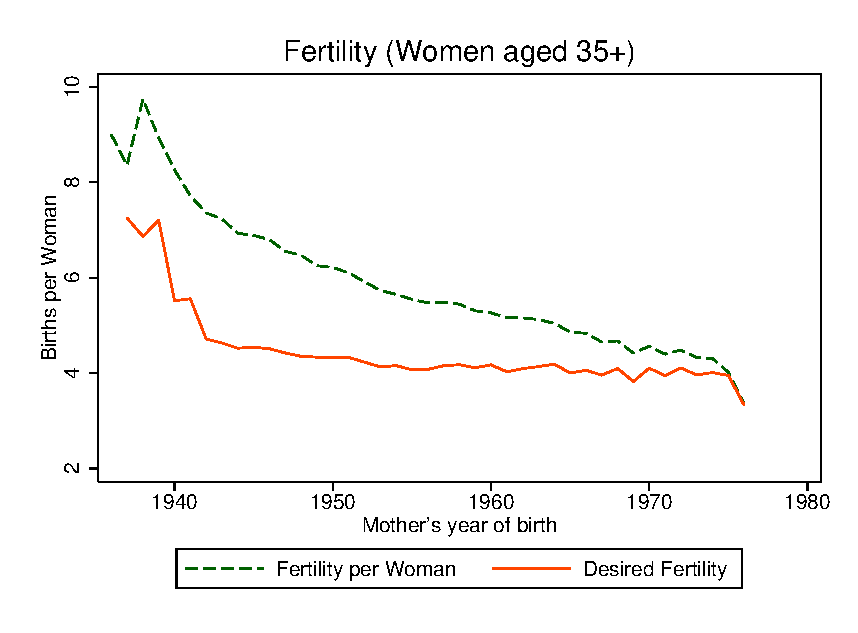
\includegraphics[scale=0.53]{\twinfolder/Figures/ferttrend_35_all.eps}
  \caption{Trends in Fertility}
  \label{TWINfig:fertrend}
\end{subfigure}%
\begin{subfigure}{.5\textwidth}
  \centering
  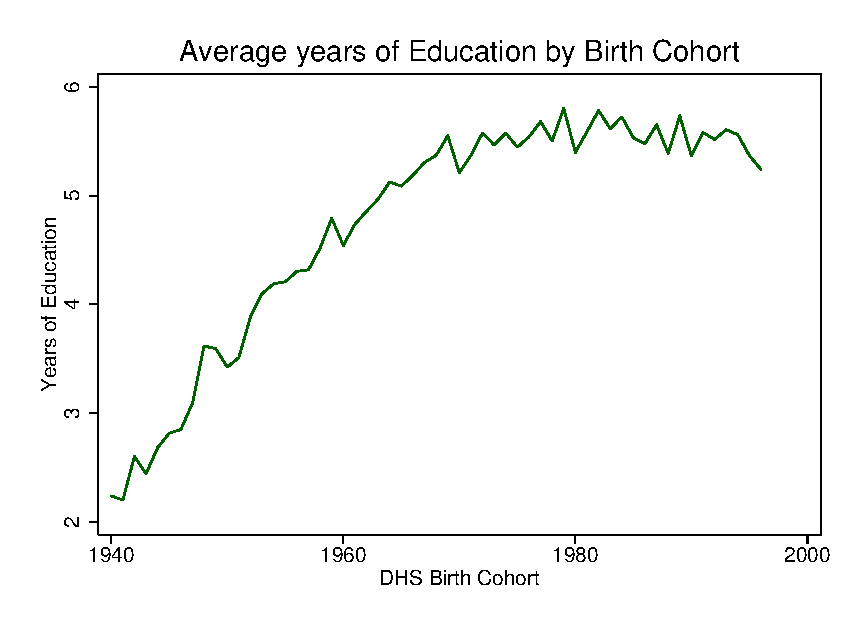
\includegraphics[scale=0.52]{\twinfolder/Figures/eductrend_all.eps}
  \caption{Trend in Education}
  \label{TWINfig:eductrend}
\end{subfigure}
\caption{Education and Fertility}
\label{TWINfig:trends}
\floatfoot{Note to figure \ref{TWINfig:trends}: Cohorts are made up of all individuals 
from the DHS who are over 35 years (for fertility), and over 15 years (for education).  
In each case the sample is restricted to those who have approximately completed fertility 
and education respectively.}
\end{figure}
\vspace{1cm}

\begin{figure}[htpb!]
\begin{center}
\caption{Proportion of Twins of All Births (USA)}
\label{TWINfig:bord}
\includegraphics[scale=0.92]{\twinfolder/Figures/USTwinFLE.eps} 
\end{center}
\end{figure}

\begin{figure}[htpb!]
\begin{center}
\caption{Twin Births and Total Fertility}
\label{TWINfig:births}
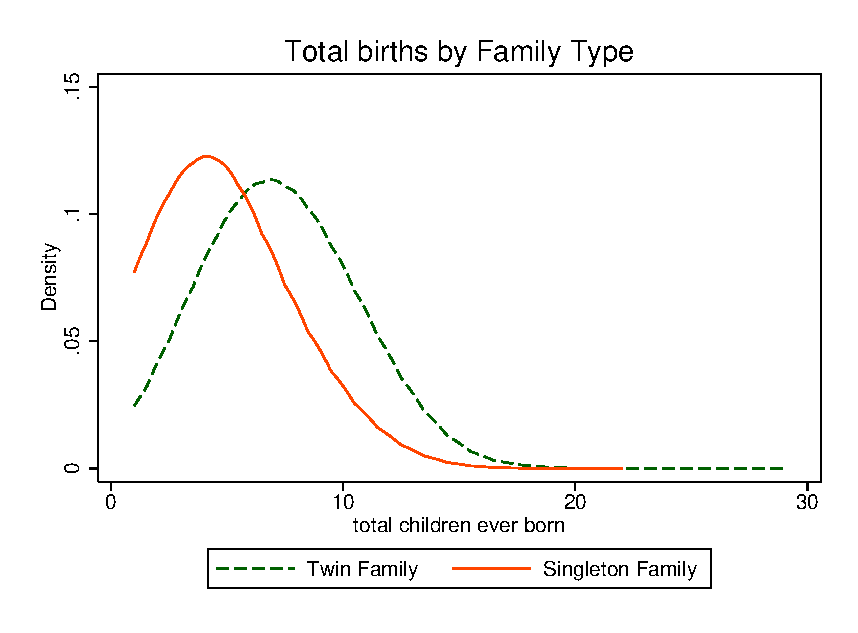
\includegraphics[scale=0.92]{\twinfolder/Figures/famsize.eps} 
\end{center}
\end{figure}

\begin{figure}[htpb!]
\begin{center}
\caption{Proportion of Twins by Birth Order}
\label{TWINfig:bord}
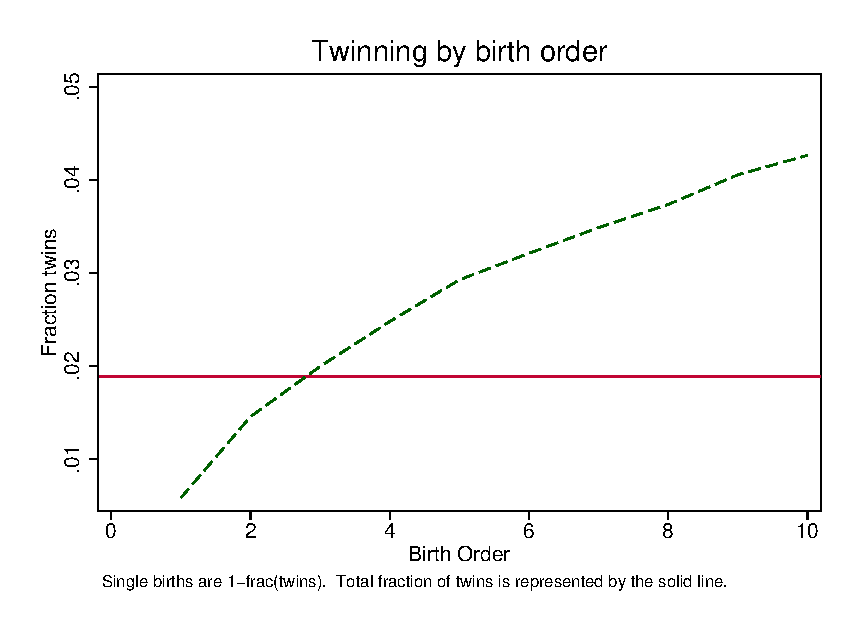
\includegraphics[scale=0.92]{\twinfolder/Figures/twinbybord.eps} 
\end{center}
\end{figure}

\begin{figure}[htpb!]
\begin{center}
\caption{Intra- and Inter-country trends: height and twinning}
\label{TWINfig:arrows}
\includegraphics[scale=0.86]{\twinfolder/Figures/height_country.eps} 
\end{center}
\end{figure}

%\begin{figure}[htpb!]
%\begin{center}
%\caption{Distribution of Ideal Family Size}
%\label{TWINfig:ideal}
%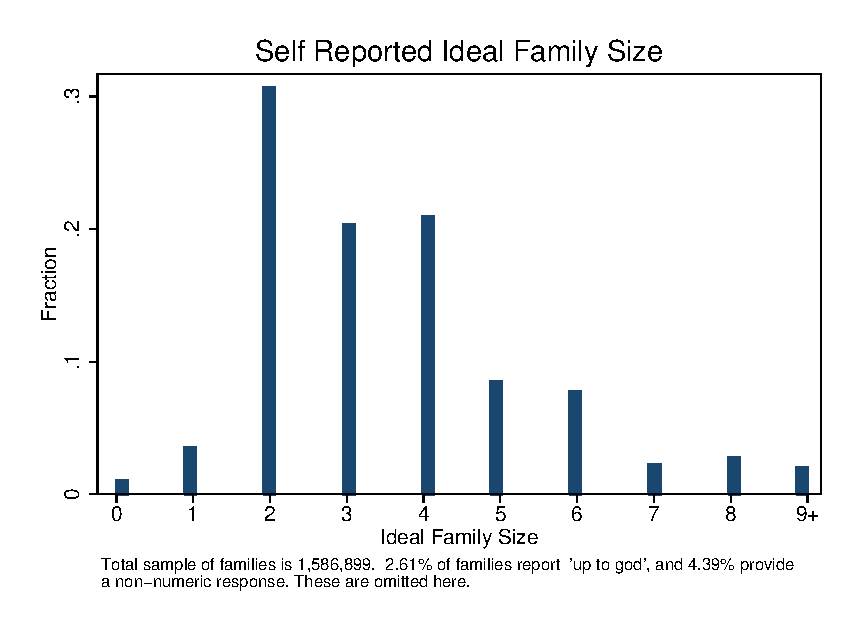
\includegraphics[scale=0.92]{\twinfolder/Figures/idealfamsize.eps} 
%\end{center}
%\end{figure}

%\begin{figure}[htpb!]
%\begin{center}
%\caption{Ideal and Actual Fertility}
%\label{TWINfig:idealactual}
%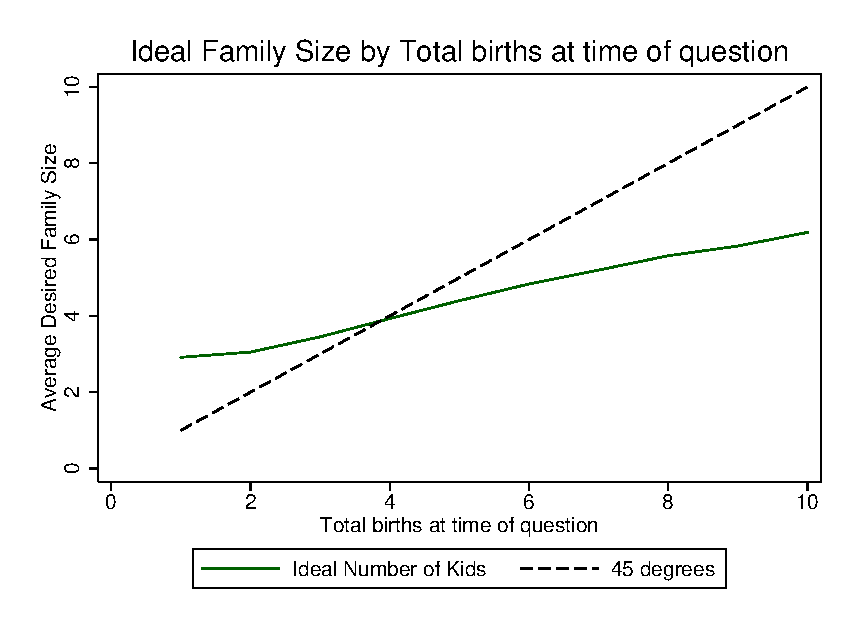
\includegraphics[scale=0.92]{\twinfolder/Figures/idealfam_fert.eps} 
%\end{center}
%\end{figure}

\begin{figure}[htpb!]
\begin{center}
\caption{Relaxing Strict Exogeneity (two plus)}
\label{TWINfig:ltz2}
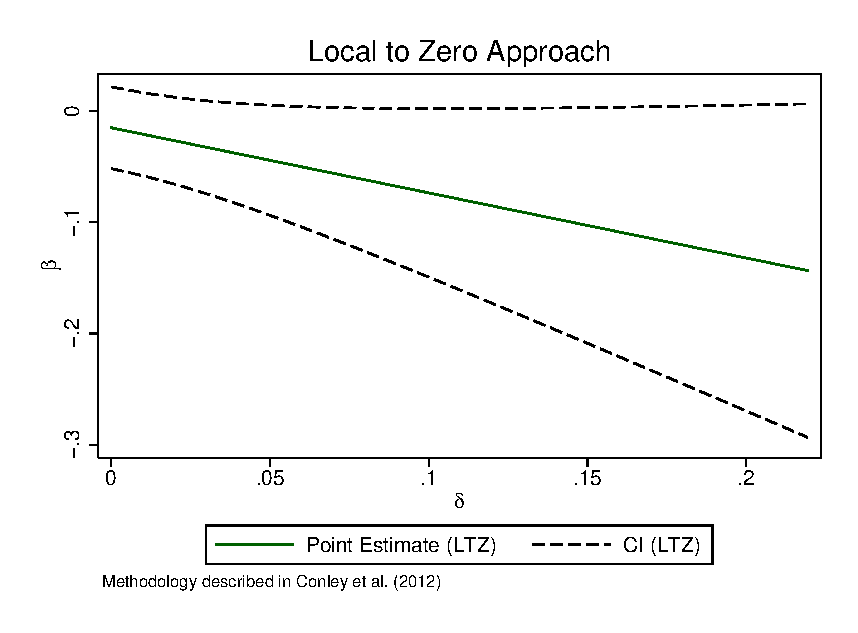
\includegraphics[scale=0.88]{\twinfolder/Figures/LTZ_two.eps}
\vspace{-8mm}
\floatfoot{Note to figure \ref{TWINfig:ltz2}: See note to Figure \ref{TWINfig:ltz3}}
\end{center}
\end{figure}

\begin{figure}[htpb!]
\begin{center}
\caption{Relaxing Strict Exogeneity (three plus)}
\label{TWINfig:ltz3}
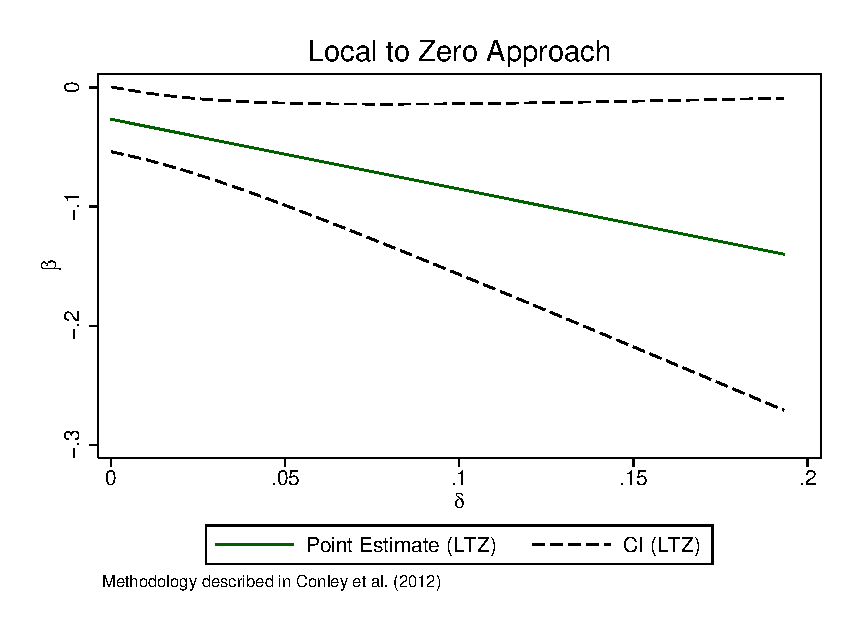
\includegraphics[scale=0.88]{\twinfolder/Figures/LTZ_three.eps} 
\floatfoot{Note to figure \ref{TWINfig:ltz3}: Confidence intervals and point estimates 
are calculated according to \citet{Conleyetal2012}.  Estimates reflect a range of priors 
regarding the validity of the exclusion restriction required to consistently estimate 
$\hat\beta_{fert}$ using twinning in a 2SLS framework.  The local to zero (LTZ) 
approach applied here assumes that $\gamma$, the sign on the instrument when included
in the first stage, is distributed $\gamma\sim U(0,\delta)$.  Further discussion 
is provided in the body of the text and table \ref{TWINtab:Conley}.}
\end{center}
\end{figure}




\clearpage
\section*{Tables}
\clearpage


\bibliography{./BiBBase1}

\newpage
\appendix
\section*{Appendices}
\section{Data Appendix}
\section{Appendix Tables}
\section{Appendix Figures}
\setcounter{figure}{0}
\renewcommand{\thefigure}{A\arabic{figure}}

\begin{figure}[htpb!]
\begin{center}
\caption{Height and Selective Survival}
\label{TWINfig:bord}
\includegraphics[scale=0.92]{\twinfolder/Figures/MMRcuts.eps} 
\end{center}
\end{figure}






\end{spacing}
\end{document}


%Short.

